\documentclass[8pt,letterpaper]{article}
\author{SJ}
\usepackage{graphicx}
\usepackage{caption}
\usepackage{subcaption}
\usepackage{hyperref}
\hypersetup{
    colorlinks=true,
    linkcolor=blue,
    filecolor=magenta,      
    urlcolor=cyan,
}
\setcounter{secnumdepth}{0}
\begin{document}

\title{Gaussian randomization in a random walker and world weight}
\maketitle
\begin{figure}[h]
\centering
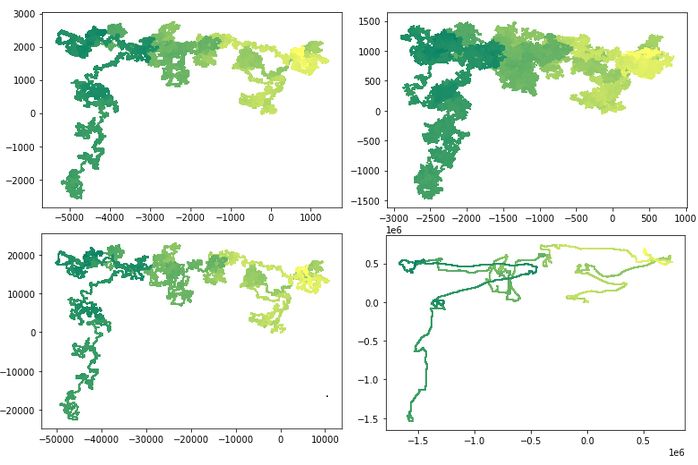
\includegraphics[scale = 0.7]{Images/frontpage.png}
\end{figure}

\newpage{}
\tableofcontents
\section{Introduction}
A short introduction to an expansion to the random walker made before, a walker with gaussian randomization. The file SingleStep\_Map\_generator.pdf goes into detail about the idea of the program and why it wont be used, this is merely a practice exercise in understanding randomization.

\section{What Are Gaussian Randomizers}
This section is oversimplified as Gaussian randomizers are just a means to an end for this walker. There are a lot of good tutorials on gaussian functions and randomizers online here is a simple tutorial for example \url{https://www.youtube.com/watch?v=IIuXF5QRBTY}. 

Gaussian functions create vaues in a way they would occur in nature, with values that happen more often and values that dont happen often. naturally they occur in a bell curve(\ref{fig:bell_curve.png}). Things like creature heights and even test scores ofen occur with such a curve .


\begin{figure}[!h]
	\centering
	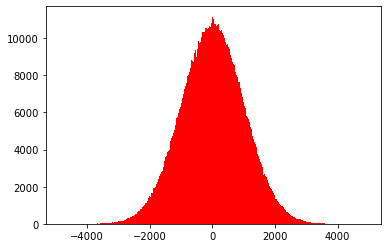
\includegraphics[scale = 0.7]{Images/bell_curve.png}
	\caption{A standard bell curve}
	\label{fig:bell_curve.png}
\end{figure}

\section{Let's Get gaussian}

A Gaussian randomizer is added to the walker to set the distance the walker can jump to a direction in one turn. The pyton version of gaussian randomizer returns floats which I convert to ints in order to make the table with all numbers not to big to run.

Where the first version only jumped 1 in any direction this version jumps from a standard . This version picks a direction and jumps a distance using the follwing python formula for both x and y.
The colouring formula is the same as in the previous version as the random walker. The formula is the following, the only change in the working version being that we cast it into an int.
\begin{equation}
	\label{eq:RandomWalkerFormula}
	n1 = gauss(self.world\_compression * -self.x\_change\_previous,10)
\end{equation}
Gauss is a randomizer in python that picks random numbers based on a bell curve. The 10 is the standard deviation and the $self.world\_compression * -self.x\_change\_previous$ is the starting point, always starting out at zero.

The x\_change zero is a check what the result of the formula was the previous time we ran it. The world\_compression is a number between 1 and -1 that decides how compressed(how close together is the landmass.) the world generation is. if the number is larger then 0 the world becomes more compressed due to the prevous sum being removed from the formula. If the number is lower then zero the world becomes less compressed. in the figure below(\ref{fig:3_worlds}) the landmass diffrent forms of landmass are shown.

\begin{figure}[!h]
\centering

	\begin{subfigure}[b]{0.32\textwidth}
		\centering
		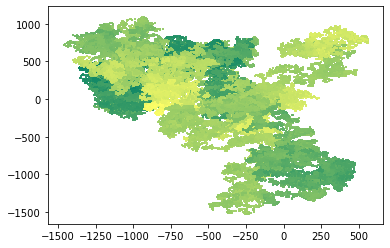
\includegraphics[width=\textwidth]{Images/fat_landmass1.png}
		\caption{World\_compression = 1}
	\end{subfigure}
	\begin{subfigure}[b]{0.32\textwidth}
		\centering
		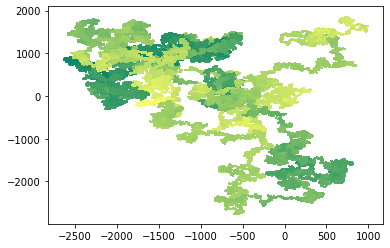
\includegraphics[width=\textwidth]{Images/diet_landmass1.png}
		\caption{World\_compression = 0}
	\end{subfigure}
	\begin{subfigure}[b]{0.32\textwidth}
		\centering
		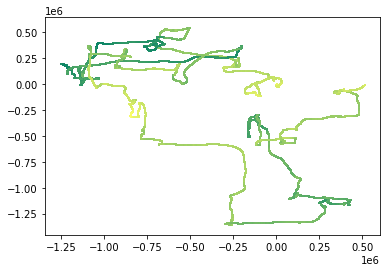
\includegraphics[width=\textwidth]{Images/skinny_landmass1.png}
		\caption{World\_compression = -1}
	\end{subfigure}
\caption{several world compressions shown}
\label{fig:3_worlds}
\end{figure}
\section{conclusion}
The conclusion drawn from this expansion is the following, adding complexety to the movement algortihm makes control of world generation a lot easier. The final version of the randomizer needs to have a good balance between complexity and control needs to be researched in the final version.
\end{document}\





